%%%%%%%%%%%%%%%%%%%%%%%%%%%%%%%%%%%%%%%%%
% Copyright 2018 Tactical Computing Laboratories, LLC
% See LICENSE for licensing details
%%%%%%%%%%%%%%%%%%%%%%%%%%%%%%%%%%%%%%%%%

%----------------------------------------------------------------------------------------
%	PACKAGES AND DOCUMENT CONFIGURATIONS
%----------------------------------------------------------------------------------------

\documentclass{article}

% Package includes

\usepackage{graphicx}
\usepackage{geometry}
\usepackage{array}
\usepackage{colortbl}
\usepackage{hyperref}
\usepackage{placeins}
\usepackage{longtable}
\usepackage{multirow}
\usepackage{float}
\usepackage{caption}

\usepackage{natbib} % Required to change bibliography style to APA
\usepackage{amsmath} % Required for some math elements 
\usepackage[boxed]{algorithm2e} % required for algorithms
\usepackage{fancyhdr}
\RequirePackage{epstopdf}
\RequirePackage{tabularx}
\RequirePackage{xstring}
\RequirePackage{hyperref}
\RequirePackage{fancyhdr}

\usepackage[olditem,oldenum]{paralist}

\usepackage[xindy,toc]{glossaries}
\usepackage[xindy]{imakeidx}
% Setup margins

\setlength{\topmargin}{-0.5in}
\setlength{\textheight}{9in}
\setlength{\oddsidemargin}{0in}
\setlength{\evensidemargin}{0in}
\setlength{\textwidth}{6.5in}

% Useful macros

\newcommand{\note}[1]{{\bf [ NOTE: #1 ]}}
\newcommand{\fixme}[1]{{\bf [ FIXME: #1 ]}}
\newcommand{\todo}[1]{\marginpar{\footnotesize #1}}

\newcommand{\wunits}[2]{\mbox{#1\,#2}}
\newcommand{\um}{\mbox{$\mu$m}}
\newcommand{\xum}[1]{\wunits{#1}{\um}}
\newcommand{\by}[2]{\mbox{#1$\times$#2}}
\newcommand{\byby}[3]{\mbox{#1$\times$#2$\times$#3}}

\newlength\savedwidth
\newcommand\whline[1]{%
  \noalign{%
    \global\savedwidth\arrayrulewidth\global\arrayrulewidth 1.5pt%
  }%
  \cline{#1}%
  \noalign{\vskip\arrayrulewidth}%
  \noalign{\global\arrayrulewidth\savedwidth}%
}

% Custom list environments

\newenvironment{tightlist}
{\begin{itemize}
 \setlength{\parsep}{0pt}
 \setlength{\itemsep}{-2pt}}
{\end{itemize}}

\newenvironment{titledtightlist}[1]
{\noindent
 ~~\textbf{#1}
 \begin{itemize}
 \setlength{\parsep}{0pt}
 \setlength{\itemsep}{-2pt}}
{\end{itemize}}

\newenvironment{commentary}
{ \vspace{-0.2in}
  \begin{quotation}
  \noindent
  \small \em
  \rule{\linewidth}{1pt}\\
}
{ 
  \end{quotation}
  \vspace{-0.2in}
}

\newenvironment{samepage-commentary}
{\begin{samepage} \begin{commentary}}
{\end{commentary} \end{samepage}}

% Other commands and parameters

\pagestyle{myheadings}
\setlength{\parindent}{0in}
\setlength{\parskip}{10pt}
\sloppy

% Commands for register format figures.

% New column types to use in tabular environment for instruction formats.
% Allocate 0.18in per bit.
\newcolumntype{I}{>{\centering\arraybackslash}p{0.18in}}
% Two-bit centered column.
\newcolumntype{W}{>{\centering\arraybackslash}p{0.36in}}
% Three-bit centered column.
\newcolumntype{F}{>{\centering\arraybackslash}p{0.54in}}
% Four-bit centered column.
\newcolumntype{Y}{>{\centering\arraybackslash}p{0.72in}}
% Five-bit centered column.
\newcolumntype{R}{>{\centering\arraybackslash}p{0.9in}}
% Six-bit centered column.
\newcolumntype{S}{>{\centering\arraybackslash}p{1.08in}}
% Seven-bit centered column.
\newcolumntype{O}{>{\centering\arraybackslash}p{1.26in}}
% Eight-bit centered column.
\newcolumntype{E}{>{\centering\arraybackslash}p{1.44in}}
% Ten-bit centered column.
\newcolumntype{T}{>{\centering\arraybackslash}p{1.8in}}
% Twelve-bit centered column.
\newcolumntype{M}{>{\centering\arraybackslash}p{2.2in}}
% Sixteen-bit centered column.
\newcolumntype{K}{>{\centering\arraybackslash}p{2.88in}}
% Twenty-bit centered column.
\newcolumntype{U}{>{\centering\arraybackslash}p{3.6in}}
% Twenty-bit centered column.
\newcolumntype{L}{>{\centering\arraybackslash}p{3.6in}}
% Twenty-five-bit centered column.
\newcolumntype{J}{>{\centering\arraybackslash}p{4.5in}}

\newcommand{\instbit}[1]{\mbox{\scriptsize #1}}
\newcommand{\instbitrange}[2]{~\instbit{#1} \hfill \instbit{#2}~}
\newcommand{\reglabel}[1]{\hfill {\tt #1}\hfill\ }

\newcommand{\wiri}{\textbf{WIRI}}
\newcommand{\wpri}{\textbf{WPRI}}
\newcommand{\wlrl}{\textbf{WLRL}}
\newcommand{\warl}{\textbf{WARL}}

\newcommand\concat{+\kern-0.5ex+}
\newcommand\regpair[2]{(\textit{#1}\concat{}\textit{#2})}

\makeglossaries


%\usepackage[margin=1.0in]{geometry}
%\usepackage[version=3]{mhchem} % Package for chemical equation typesetting
%\usepackage{siunitx} % Provides the \SI{}{} and \si{} command for typesetting SI units
%\usepackage{graphicx} % Required for the inclusion of images
%\usepackage{natbib} % Required to change bibliography style to APA
%\usepackage{amsmath} % Required for some math elements 
%\usepackage[boxed]{algorithm2e} % required for algorithms
%\usepackage{fancyhdr}
%\RequirePackage{epstopdf}
%\RequirePackage{tabularx}
%\RequirePackage{xstring}
%\RequirePackage{hyperref}
%\RequirePackage{fancyhdr}

%-- setup paragraphs and margins
\setlength{\parindent}{1em}
\setlength{\parskip}{1em}


%-- setup hyperlinks
\hypersetup{
  colorlinks=true,
  linktoc=all,
  linkcolor=black,
  citecolor=black,
  urlcolor=black
}
%--

\setlength\parindent{0pt} % Removes all indentation from paragraphs


\renewcommand{\labelenumi}{\alph{enumi}.} % Make numbering in the enumerate environment by letter rather than number (e.g. section 6)

\pagestyle{fancy}
\lhead{}
\chead{\textbf{xBGAS Architecture Extension Specification}}  % -- classification
\rhead{}
\cfoot{} %-- format: TR YYYY-RRR-V.V; y = year; r = report; v = version
\lfoot{\textbf{xBGAS 0.0.6}}  % -- classification
\rfoot{\thepage}      % -- page number

%\usepackage{times} % Uncomment to use the Times New Roman font

%----------------------------------------------------------------------------------------
%	DOCUMENT INFORMATION
%----------------------------------------------------------------------------------------

\title{\textbf{RISC-V Extended Addressing\\Architecture Extension Specification\\Codenamed: xBGAS}} % Title

%\author{John \textsc{Leidel}, David \textsc{Donofrio}, Farzad \textsc{Fatollahi-Fard}}
\date{} % Date for the report

\begin{document}

\begin{figure}
\vspace{2in}
\begin{center}

\includegraphics[width=3in]{figures/xbgas.pdf} % Include the logo
\end{center}
\end{figure}

\maketitle % Insert the title, author and date

\thispagestyle{fancy}

\begin{center}
\begin{tabular}{l r}
Date: & \today \\
Version: & 0.0.6 \\ % Date the experiment was performed
Authors: & John Leidel\\
& David Donofrio\\
& Farzad Fatollahi-Fard\\
& Xi Wang
\end{tabular}
\end{center}

\clearpage

\tableofcontents

\clearpage

%----------------------------------------------------------------------------------------
%	DEFINITIONS
%----------------------------------------------------------------------------------------
%\section*{Terms}
%\label{sec:terms}


%----------------------------------------------------------------------------------------
%       List of Figures
%----------------------------------------------------------------------------------------

\clearpage
\listoffigures
%\lstlistoflistings
\listoftables
%\listofalgorithms
\clearpage

%----------------------------------------------------------------------------------------
%	SECTION 1
%----------------------------------------------------------------------------------------
\clearpage
\section{Introduction}

\subsection{xBGAS Overview}

The goal of the \gls{xBGAS} extension described herein is to provided \textit{extended} 
addressing capabilities beyond the core 64-bit addressing modes available in the 
base RISC-V RV64I instruction set specification.  These extensions provide up 
to 128 bits of virtual or physical address space (depending upon the target implementation) 
to implementors in the form of basic instruction extensions that utilize extended 
register sets for the 64 most significant bits of the target address.  

Note that these extensions \textbf{do not} provide an inherently flat 128-bit address space.  
Further, they do not explicitly modify the incumbent RV32I or RV64I memory access 
methodologies.  Rather, these additions are extensions to the base level specifications in order to 
permit normal, byte-aligned memory access to address spaces larger than 64-bits.  In 
this manner, users may build and execute applications that support RV32I and RV64I 
instructions without utilizing the xBGAS extensions without issue.  Further, RV32I and RV64I 
applications that are binary compatible should execute unencumbered on a system that 
complies with the xBGAS extensions described herein.

\subsection{xBGAS Extension ISA Requirements}

The xBGAS instruction set extension described herein is classified 
as a \textit{brownfield} extension with respect to the core RISC-V 
machine state.  In this manner, fits within the existing RISC-V instruction 
formats and encodings.  However, the xBGAS extension does instantiate 
additional machine state in terms of user-visible and supervisor registers.

The xBGAS specification functions as an extension to the existing RV64I~\cite{RVSpec} 
base instruction set specification (and all inherited instructions therein).  In this 
manner, the xBGAS extension is truly an extension, rather than a full expansion 
of the register \textit{XLEN} and the associated ALU.

\subsection{xBGAS Implementation Requirements}

The goal of this specification is to outline the required encoding, register extensions 
and associated supervisor level functionality required to implement the xBGAS 
RISC-V extension.  It does not, however, imply any specific required implementation 
functionality unless otherwise noted herein.  Specific topics that are deliberately 
left up to the implementor can be summarized as follows:

\begin{itemize}
\item \textbf{Caching}: This specification does not require or prohibit the use of data caching 
when operating with 128-bit addressing.  It is up to the implementor to define if/how data caching 
is present and/or utilized.  

\item \textbf{Address Encoding}: This specification does not define any specific 64-bit or 128-bit 
address encoding format beyond what is described in the base RV64I specification.  Implementors 
may choose to utilize a partitioned addressing schema, a flat schema or combinations thereof.    

\item \textbf{Scalability}: This specification does not define the scalability of the least significant 
or most significant 64-bit address words.  For example, it is well within the implementor's power to 
utilize a 48-bit base address encoding and a small number of most significant (extended) encoding bits.

\item \textbf{Extended Memory Translation}: This specification does not require the use of any 
specific paging and/or virtual to physical translation methodology.  It is up to the implementor to define 
if/how virtualized memory access is implemented for the extended addressing.

\item \textbf{Memory Controllers}: This specification does not mention, nor require any specific 
location or implementation of the memory controller (et al. downstream memory components).  It is 
up to the implementor to define how/where the memory controller is implemented based upon the 
target system architecture requirements.

\item \textbf{Memory Bus/Interconnection}: This specification does not mention, nor require any 
specific memory bus or memory interconnection infrastructure.  It is up to the implementor to define 
how the memory units are connected to the target memory device or devices.

\item \textbf{Pipeline Model}: This specification does not mention, nor require any specific 
core pipeline model.  It is up to the implementor to define how the xBGAS instructions are 
implemented.

\item \textbf{Virtualization}: This specification makes no mention of implementing a virtualization 
layer on top of xBGAS-style addressing.  Do not expect that xBGAS addressing modes will 
automatically function with pre-defined RV64I virtualization mechanisms.  This is beyond the 
scope of this document.

\item \textbf{Enclaves}: This specification makes no mention of implementating functionality 
associated with system or machine-level security enclaves.  Any security-related functionality 
required to enforce enclaves on a system with xBGAS extensions is beyond the scope 
of this document.

\end{itemize}

\subsection{xBGAS Supervisor Specification Requirements}

\subsubsection{Machine ISA Register {\tt misa}}

As noted by the supervisor specification~\cite{RVSuperSpec}, the 
\textit{misa} CSR register is an XLEN-bit \warl\ read-write register reporting 
the supported ISA by the hart.  Normally, the MXL (Machine XLEN) field 
encodes the native base integer width as shown in the supervisor specification.  
In the case of xBGAS, this value is set to represent a 64-bit base ISA (\textit{MXL=2}).  We do 
not override this value as the xBGAS implementation described herein does not 
natively modify the register width of the general purpose registers beyond 64-bits.    

\begin{figure*}[h!]
{\footnotesize
\begin{center}
\begin{tabular}{c@{}c@{}J}
\instbitrange{XLEN-1}{XLEN-2} &
\instbitrange{XLEN-3}{26} &
\instbitrange{25}{0} \\
\hline
\multicolumn{1}{|c|}{MXL[1:0] (\warl)} &
\multicolumn{1}{c|}{\wiri} &
\multicolumn{1}{c|}{Extensions[25:0] (\warl)} \\
\hline
2 & XLEN-28 & 26 \\
\end{tabular}
\end{center}
}
\vspace{-0.1in}
\caption{Machine ISA register ({\tt misa}).}
\label{misareg}
\end{figure*}

As stated in the supervisor specification, the \textbf{Extensions} field encodes the presence of the 
standard extensions via a single bit per letter of the alphabet.  Per this notional encoding, 
the ``I'' bit (bit-8) must be set for all implementations that support xBGAS.  Further, we also dictate 
that the ``X'' bit (bit-23) must be set to indicate a non-standard extension.

\begin{commentary}
Given that xBGAS is currently a non-standard extension, the ``X'' bit must be set.  However, 
portions of this specification may be integrated into the official SV128 specification 
that will become an officially supported extension.
\end{commentary}

\subsubsection{Supervisor Cause Register ({\tt scause})}

Per the supervisor specification, the {\tt scause} register is an XLEN-bit read-write register 
formatted as per Figure~\ref{scausereg}.  The xBGAS specification does not add any specific 
Exception Code values to be placed in the \wlrl\ field.  However, much in the manner of 
normal load and store operations from RV32I and RV64I, the xBGAS extension has the ability 
trigger the codes listed in Table~\ref{scauses}.   

\begin{figure*}[h!]
{\footnotesize
\begin{center}
\begin{tabular}{c@{}U}
\instbit{XLEN-1} &
\instbitrange{XLEN-2}{0} \\
\hline
\multicolumn{1}{|c|}{Interrupt} &
\multicolumn{1}{c|}{Exception Code (\wlrl)} \\
\hline
1 & XLEN-1 \\
\end{tabular}
\end{center}
}
\vspace{-0.1in}
\caption{Supervisor Cause register {\tt scause}.}
\label{scausereg}
\end{figure*}

\begin{table*}[h!]
\begin{center}
\begin{tabular}{|r|r|l|l|}

  \hline
  Interrupt & Exception Code  & Description \\
  \hline	 
  0         & 2               & Illegal instruction \\   
  0         & 3               & Breakpoint \\
  0         & 5               & Load access fault \\
  0         & 7               & Store/AMO access fault \\
  0         & 13              & Load page fault \\
  0         & 15              & Store/AMO page fault \\
  \hline
\end{tabular}
\end{center}
\caption{xBGAS Supervisor cause register ({\tt scause}) values after trap.}
\label{scauses}
\end{table*}

%----------------------------------------------------------------------------------------
%	SECTION 2
%----------------------------------------------------------------------------------------
\clearpage
\section{xBGAS Machine Organization}

\subsection{xBGAS Extended Addressing Logic}

At the core of the xBGAS implementation is the ability to utilize existing RV64I 
binary blobs without issue.  In this manner, the xBGAS extension makes use 
of the base RV64I register length, memory operations and ALU functionality.  
The key portions of the xBGAS functionality and associated address mode 
is implemented via an extended register file that is mapped to a series 
of base registers as well as a set of xBGAS-specific instructions to perform 
standard load, store and register manipulation of extended 128-bit addresses.  We 
see this extended register set depicted in Figure~\ref{fig:machineorganization}.  

\begin{figure}[h!]
\begin{center}
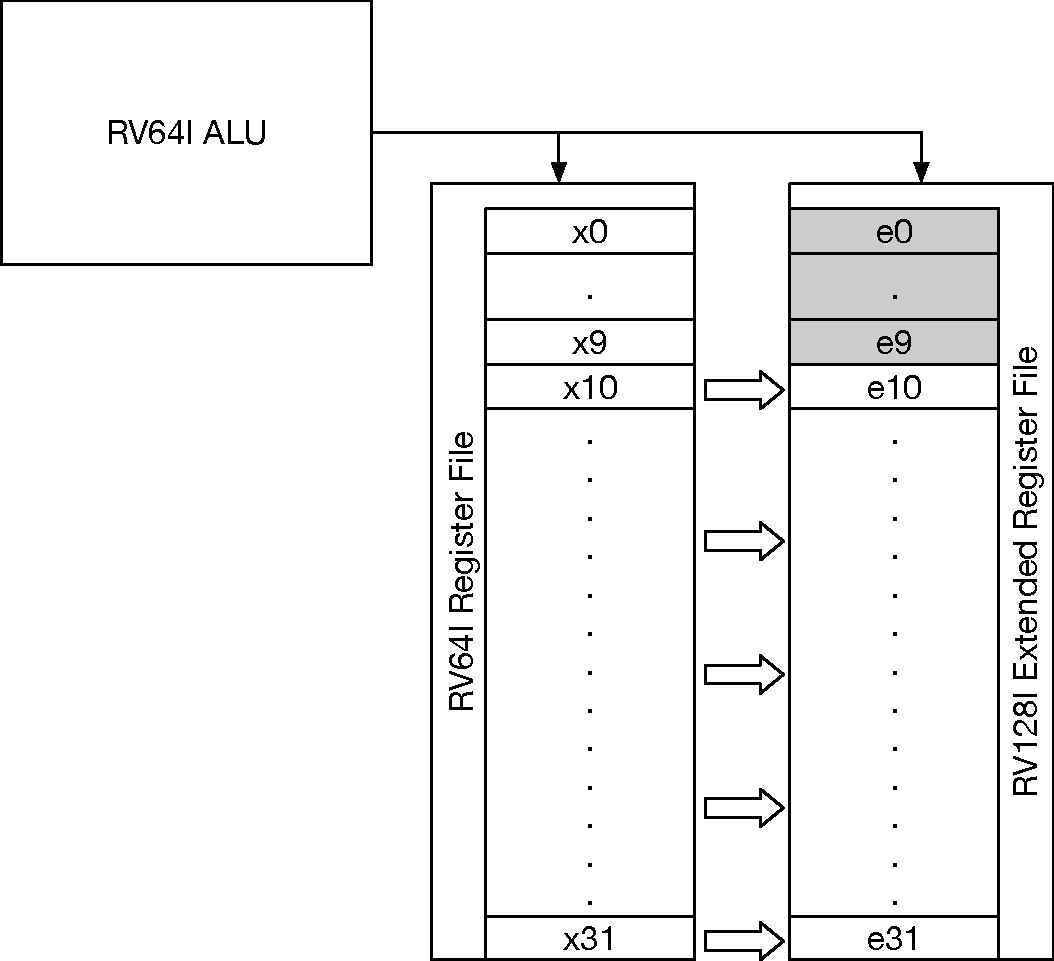
\includegraphics[width=3in]{figures/rv128imachorg.pdf}
\caption{xBGAS Machine Organization}
\label{fig:machineorganization}
\end{center}
\end{figure}

In the aforementioned figure, note the specific mapping of base registers 
(\textit{xN}) to extended registers(\textit{eN}).  For each of the base 
registers beginning at index \textit{0}, we map a complementary extended 
register at the same index.  In this manner, xBGAS memory operations 
utilize both the base and extended registers at the target index in the process 
of formulating the extended addressing schema.  However, also note that 
the first ten indices (\textit{0-9}) cannot be utilized for addressing.  These 
indices are reserved for operations in the memory translation layer.  This is 
analogous to the first ten indices in the general purpose register file 
that are specifically allocated to various operations associated with instruction 
handling (\textit{sp}), frame handling (\textit{fp}), context save/restore 
and hard encoding (\textit{zero/x0}).  As a result, these registers cannot be 
utilized in generating extended addresses for xBGAS memory operations.  
Any attempt to utilize extended registers below index \textit{10} will 
result in an exception.    

\begin{figure}[h!]
\begin{center}
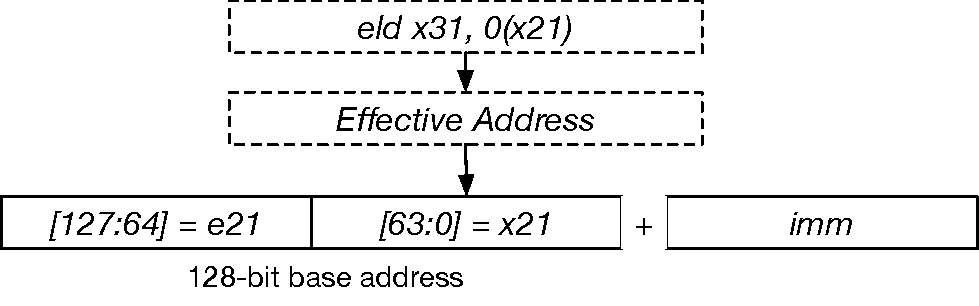
\includegraphics[width=3in]{figures/effectiveaddress.pdf}
\caption{xBGAS Effective Address Calculation}
\label{fig:effectiveaddr}
\end{center}
\end{figure}

Given the aforementioned machine organization, we may also describe the xBGAS addressing methodology.  
Figure~\ref{fig:effectiveaddr} depicts how xBGAS load and store operations generate effective addresses.  For each 
given xBGAS memory operation, we see that the base register index encoded in the instruction payload references 
the base register file.  This 64-bit value (\textit{x21} in the figure) represents the least significant 64 bits of the effective 
xBGAS address.  In addition to the base register, the instruction also utilizes the 64-bit value from the complementary 
extended register, \textit{e21}, for the most significant 64 bits of the effective address.  Finally, we utilize the immediate 
value in the instruction payload for any potential offset calculations.

\subsection{xBGAS Register State}
In addition to the registers defined as a part of the base RISC-V IMAFD ISA, we define an additional set of registers for the xBGAS extension.  The register extension is defined in terms of User-Visible, Supervisor and Machine-State registers.  User-Visible registers are those that can be read and written from normal user instructions.  Supervisor registers are those that can only be read and written from supervisor-privileged instructions.  Machine-State registers cannot be read or written from any instruction space.  Rather, these registers are implicitly modified during the normal operation of the core.     

\subsubsection{User-Visible Registers} 
The xBGAS extension adds a series of \emph{extended} registers to the list of user-visible registers.  Each extended register is an unsigned 64-bit register that contains the most significant 64-bits of a 128-bit memory address.  In this manner, normal 64-bit and 32-bit memory operations (RV64I and RV32I respectively) are effectively unchanged.  The xBGAS extended registers can only be utilized for memory operations when utilizing xBGAS load and store operations.  Further, extended registers can only be read from and written to from xBGAS Address Management Instructions (Section~\ref{sec:AddressManagementInstructions}).   

\begin{center}
\makebox[\textwidth][s]{63 0}
\framebox[\textwidth][c]{E\textit{n}}
\end{center}

\subsubsection{Supervisor Registers}

We make use of no new supervisor registers beyond what is 
currently defined in the RV64I specification.  

\subsubsection{Machine-State Registers}

We make use of no new machine-state registers beyond what is 
currently defined in the RV64I specification.  

\newpage
\subsubsection{XBGAS Register Indexing}
A summary of the permissible xBGAS register indices, their assembly 
mnemonics and associated base register mappings is outlined as follows.  
Note the explicit negation of specific extended registers in order to prohibit 
erroneous use of the stack, frame and other core ABI dependencies.  The register 
indexing follows the base RV64I encoding standard with 5-bit indices that 
map directly to complementary base register encodings.  

\begin{center}
\begin{tabular}{| c | c | c | c | c |}
\hline
Register & xBGAS Mapping & Index & Description & ABI Name\\ \hline
\hline
e0-e9 & x0-x9 & 0b0000-0b1001 & Utilized for memory translation & e0-e9\\
\hline
e10-11 & x10-11 & 0b1010-0b1011 & Function arguments/return values & e10-11\\
\hline
e12-17 & x12-17 & 0b1100-0b10001 & Function arguments & e12-17\\
\hline
e18-27 & x18-27 & 0b10010-0b11011 & Saved registers & e18-27\\
\hline
e28-31 & x28-31 & 0b11100-0b11111 & Temporaries & e28-31\\
\hline
\end{tabular}
\end{center}

%----------------------------------------------------------------------------------------
%	SECTION 3
%----------------------------------------------------------------------------------------
\newpage
\section{xBGAS Instruction Set Extension}

%------- INTEGER LOAD/STORE INSTRUCTIONS
\subsection{Integer Load/Store Instructions}

xBGAS load and store instructions are encoded in the manner as the standard RV32I and 
RV64I load and store instructions.  Load instructions are encoded in the I-type format and store 
instructions are encoded in the S-type format.  The effective byte address is obtained by adding 
register pair \textit{rs1} + \textit{ext1} to the sign-extended 12-bit offset.  Note that base address 
(\textit{rs1} + \textit{ext1}) are obtained by combining the values of the base register \textit{rs1} 
and its complementary extended registers \textit{ext1}.  The least significant 64 bits of the address
[63-0] are encoded in the base register.  The most significant 64 bits of the address [127-64] 
are encoded in the extended register.  

\vspace{-0.4in}
\begin{center}
\begin{tabular}{M@{}R@{}S@{}R@{}O}
\\
\instbitrange{31}{20} &
\instbitrange{19}{15} &
\instbitrange{14}{12} &
\instbitrange{11}{7} &
\instbitrange{6}{0} \\
\hline
\multicolumn{1}{|c|}{imm[11:0]} &
\multicolumn{1}{c|}{rs1} &
\multicolumn{1}{c|}{funct3} &
\multicolumn{1}{c|}{rd} &
\multicolumn{1}{c|}{opcode} \\
\hline
12 & 5 & 3 & 5 & 7 \\
offset[11:0] & base & width & dest & LOAD \\
\end{tabular}
\end{center}

\vspace{-0.2in}
\begin{center}
\begin{tabular}{O@{}R@{}R@{}S@{}R@{}O}
\\
\instbitrange{31}{25} &
\instbitrange{24}{20} &
\instbitrange{19}{15} &
\instbitrange{14}{12} &
\instbitrange{11}{7} &
\instbitrange{6}{0} \\
\hline
\multicolumn{1}{|c|}{imm[11:5]} &
\multicolumn{1}{c|}{rs2} &
\multicolumn{1}{c|}{rs1} &
\multicolumn{1}{c|}{funct3} &
\multicolumn{1}{c|}{imm[4:0]} &
\multicolumn{1}{c|}{opcode} \\
\hline
7 & 5 & 5 & 3 & 5 & 7 \\
offset[11:5] & src & base & width & offset[4:0] & STORE \\
\end{tabular}
\end{center}


%-- extended 128bit load
\subsubsection{elq rd, imm(rs1)}
Load a 128-bit word from the address formed by adding the immediate value to the 
128-bit address at \textit{ext1+rs1}.  Store the results in \textit{rd+extd}.  The most 
significant 64-bits [127-64] are stored in the extended register \textit{extd}.  The least 
significant 64-bits are stored in the base register \textit{rd}.  The effective 
address is calculated as follows: 

\begin{equation}
Effective = addr([127-64](ext1) \cdot [63-0](rs1))+imm
\end{equation}

\begin{commentary}
The xBGAS extension explicitly contains a definition for loading 128-bit values.  
This is specified in order to provide support for handling fully-qualified (base 
address + extended) xBGAS addresses in the absence of the RV128I extension.  However, 
if the microarchitecture supports RV128I, the \textit{ELQ} instruction can be aliased 
to the \textit{LQ} instruction.
\end{commentary}


%-- extended 64bit load
\subsubsection{eld rd, imm(rs1)}
Load a 64-bit word from the address formed by adding the immediate value to the 
128-bit address at \textit{ext1+rs1}.  Store the results in \textit{rd}.  The effective 
address is calculated as follows: 

\begin{equation}
Effective = addr([127-64](ext1) \cdot [63-0](rs1))+imm
\end{equation}

%-- extended 32bit load
\subsubsection{elw rd, imm(rs1)}
Load a 32-bit word from the address formed by adding the immediate value to the 
128-bit address at \textit{ext1+rs1}.  Store the results in \textit{rd}.  The effective 
address is calculated as follows: 

\begin{equation}
Effective = addr([127-64](ext1) \cdot [63-0](rs1))+imm
\end{equation}

%-- extended 16bit load
\subsubsection{elh rd, imm(rs1)}
Load a 16-bit word from the address formed by adding the immediate value to the 
128-bit address at \textit{ext1+rs1}.  Store the results in \textit{rd}.  The effective 
address is calculated as follows: 

\begin{equation}
Effective = addr([127-64](ext1) \cdot [63-0](rs1))+imm
\end{equation}

%-- extended 16bit load + zero extend
\subsubsection{elhu rd, imm(rs1)}
Load a 16-bit word from the address formed by adding the immediate value to the 
128-bit address at \textit{ext1+rs1}.  Store the results in \textit{rd}.  
 The target register is zero extended to 64-bits.  The effective 
address is calculated as follows: 

\begin{equation}
Effective = addr([127-64](ext1) \cdot [63-0](rs1))+imm
\end{equation}

%-- extended 8bit load
\subsubsection{elb rd, imm(rs1)}
Load an 8-bit word from the address formed by adding the immediate value to the 
128-bit address at \textit{ext1+rs1}.  Store the results in \textit{rd}.  The effective 
address is calculated as follows: 

\begin{equation}
Effective = addr([127-64](ext1) \cdot [63-0](rs1))+imm
\end{equation}

%-- extended 8bit load + zero extend
\subsubsection{elbu rd, imm(rs1)}
Load an 8-bit word from the address formed by adding the immediate value to the 
128-bit address at \textit{ext1+rs1}.  Store the results in \textit{rd}.  
 The target register is zero extended to 64-bits.  The effective 
address is calculated as follows: 

\begin{equation}
Effective = addr([127-64](ext1) \cdot [63-0](rs1))+imm
\end{equation}

%-- extended register load
\subsubsection{ele extd, imm(rs1)}
Load a 64-bit word from the address formed by adding the immediate value to the 
64-bit address at \textit{rs1}.  Store the results in the extended register \textit{extd}.  
This operation is designed to be utilized for context restore operations.  The effective 
address is calculated as follows: 

\begin{equation}
Effective = addr(rs1)+imm
\end{equation}

%-- extended 128bit store
\subsubsection{esq rs1, imm(rs2)}
Store a 128-bit word using the value in the register pair \textit{rs1+ext1} 
as the source to the 128-bit address formed by adding the immediate value to 
the 128-bit address at \textit{ext2+rs2}.  The most significant 64-bits of the source 
are stored in the extended register at \textit{ext1} and the least significant 64-bits of the source 
are stored in the base register at \textit{rs1}.  The effective address is calculated 
as follows:  

\begin{equation}
Effective = addr([127-64](ext2) \cdot [63-0](rs2))+imm
\end{equation}

\begin{commentary}
The xBGAS extension explicitly contains a definition for storing 128-bit values.  
This is specified in order to provide support for handling fully-qualified (base 
address + extended) xBGAS addresses in the absence of the RV128I extension.  However, 
if the microarchitecture supports RV128I, the \textit{ESQ} instruction can be aliased 
to the \textit{SQ} instruction.
\end{commentary}

%-- extended 64bit store
\subsubsection{esd rs1, imm(rs2)}
Store a 64-bit word using the value in \textit{rs1} as the source 
to the 128-bit address formed by adding the immediate value to the 
128-bit address at \textit{ext2+rs2}.  The effective address is calculated 
as follows: 

\begin{equation}
Effective = addr([127-64](ext2) \cdot [63-0](rs2))+imm
\end{equation}

%-- extended 32bit store
\subsubsection{esw rs1, imm(rs2)}
Store a 32-bit word using the value in \textit{rs1} as the source 
to the 128-bit address formed by adding the immediate value to the 
128-bit address at \textit{ext2+rs2}.  The effective address is calculated 
as follows: 

\begin{equation}
Effective = addr([127-64](ext2) \cdot [63-0](rs2))+imm
\end{equation}

%-- extended 16bit store
\subsubsection{esh rs1, imm(rs2)}
Store a 16-bit word using the value in \textit{rs1} as the source 
to the 128-bit address formed by adding the immediate value to the 
128-bit address at \textit{ext2+rs2}.  The effective address is calculated 
as follows: 

\begin{equation}
Effective = addr([127-64](ext2) \cdot [63-0](rs2))+imm
\end{equation}

%-- extended 8bit store
\subsubsection{esb rs1, imm(rs2)}
Store an 8-bit word using the value in \textit{rs1} as the source 
to the 128-bit address formed by adding the immediate value to the 
128-bit address at \textit{ext2+rs2}.  The effective address is calculated 
as follows: 

\begin{equation}
Effective = addr([127-64](ext2) \cdot [63-0](rs2))+imm
\end{equation}

%-- ext context save operation 
\subsubsection{ese ext1, imm(rs2)}
Store a 64-bit word using the value in \textit{ext1} as the source to the 
64-bit address formed by adding the immediate value to the 64-bit 
address as \textit{rs2+imm}.  This operation is designed to be used for 
context save operations.  The effective address is calculated as follows: 

\begin{equation}
Effective = addr(rs2)+imm
\end{equation}

\subsection{Raw Integer Load/Store Instructions}
\label{sec:RawIntegerLoadStoreInstructions}

The raw integer load and store instructions in the xBGAS specification 
are designed to permit users and compilers to generate raw, three operand 
memory operations using explicit, non-contiguous register indexing.  In this manner, 
the instruction explicitly specifies the base register as well as the extended register 
to form the full 128-bit address encoding.  The destination register is specified as 
in all other forms of the load/store instructions.  We encode these instructions 
using the standard RISC-V R-type format as shown in Figure~\ref{fig:rinst}.  

\vspace{-0.2in}
\begin{figure}[H]
\begin{center}
\setlength{\tabcolsep}{4pt}
\begin{tabular}{p{1.2in}@{}p{0.8in}@{}p{0.8in}@{}p{0.6in}@{}p{0.8in}@{}p{1in}l}
\\
\instbitrange{31}{25} &
\instbitrange{24}{20} &
\instbitrange{19}{15} &
\instbitrange{14}{12} &
\instbitrange{11}{7} &
\instbitrange{6}{0} \\
\cline{1-6}
\multicolumn{1}{|c|}{funct7} &
\multicolumn{1}{c|}{rs2} &
\multicolumn{1}{c|}{rs1} &
\multicolumn{1}{c|}{funct3} &
\multicolumn{1}{c|}{rd} &
\multicolumn{1}{c|}{opcode} &
R-type \\
\cline{1-6}
\end{tabular}
\end{center}
\caption{R-Type Instruction Format}
\label{fig:rinst}
\end{figure}


\subsubsection{erld rd, rs1, ext2}

Load an 64-bit word from the address formed by adding the immediate value to the 
128-bit address at \textit{ext2+rs1}.  Store the results in \textit{rd}.  
The effective address is calculated as follows:

\begin{equation}
Effective = addr([127-64](ext2) \cdot [63-0](rs1))
\end{equation}

\subsubsection{erlw rd, rs1, ext2}

Load an 32-bit word from the address formed by adding the immediate value to the 
128-bit address at \textit{ext2+rs1}.  Store the results in \textit{rd}.  
The effective address is calculated as follows:

\begin{equation}
Effective = addr([127-64](ext2) \cdot [63-0](rs1))
\end{equation}

\subsubsection{erlh rd, rs1, ext2}

Load an 16-bit word from the address formed by adding the immediate value to the 
128-bit address at \textit{ext2+rs1}.  Store the results in \textit{rd}.  
The effective address is calculated as follows:

\begin{equation}
Effective = addr([127-64](ext2) \cdot [63-0](rs1))
\end{equation}

\subsubsection{erlhu rd, rs1, ext2}

Load an 16-bit word from the address formed by adding the immediate value to the 
128-bit address at \textit{ext2+rs1}.  Store the results in \textit{rd}.  
 The target register is zero extended to 64-bits.  The effective 
address is calculated as follows:

\begin{equation}
Effective = addr([127-64](ext2) \cdot [63-0](rs1))
\end{equation}

\subsubsection{erlb rd, rs1, ext2}

Load an 8-bit word from the address formed by adding the immediate value to the 
128-bit address at \textit{ext2+rs1}.  Store the results in \textit{rd}.  
The effective address is calculated as follows: 

\begin{equation}
Effective = addr([127-64](ext2) \cdot [63-0](rs1))
\end{equation}

\subsubsection{erlbu rd, rs1, ext2}

Load an 8-bit word from the address formed by adding the immediate value to the 
128-bit address at \textit{ext2+rs1}.  Store the results in \textit{rd}.  
 The target register is zero extended to 64-bits.  The effective 
address is calculated as follows: 

\begin{equation}
Effective = addr([127-64](ext2) \cdot [63-0](rs1))
\end{equation}

\subsubsection{erle extd, rs1, ext2}

Load an 64-bit word from the address formed by adding the immediate value to the 
128-bit address at \textit{ext2+rs1}.  Store the results in \textit{extd}.  
The effective address is calculated as follows:

\begin{equation}
Effective = addr([127-64](ext2) \cdot [63-0](rs1))
\end{equation}

\subsubsection{ersd rs1, rs2, ext3}

Store an 64-bit word using the value in \textit{rs1} as the source 
to the 128-bit address formed by adding the values of
128-bit address at \textit{ext3+rs2}.  The effective address is calculated 
as follows: 

\begin{equation}
Effective = addr([127-64](ext3) \cdot [63-0](rs2))
\end{equation}

\subsubsection{ersw rs1, rs2, ext3}

Store a 32-bit word using the value in \textit{rs1} as the source 
to the 128-bit address formed by adding the values of
128-bit address at \textit{ext3+rs2}.  The effective address is calculated 
as follows: 

\begin{equation}
Effective = addr([127-64](ext3) \cdot [63-0](rs2))
\end{equation}

\subsubsection{ersh rs1, rs2, ext3}

Store a 16-bit word using the value in \textit{rs1} as the source 
to the 128-bit address formed by adding the values of
128-bit address at \textit{ext3+rs2}.  The effective address is calculated 
as follows: 

\begin{equation}
Effective = addr([127-64](ext3) \cdot [63-0](rs2))
\end{equation}

\subsubsection{ersb rs1, rs2, ext3}

Store an 8-bit word using the value in \textit{rs1} as the source 
to the 128-bit address formed by adding the values of
128-bit address at \textit{ext3+rs2}.  The effective address is calculated 
as follows: 

\begin{equation}
Effective = addr([127-64](ext3) \cdot [63-0](rs2))
\end{equation}

\subsubsection{erse ext1, rs2, ext3}

Store a 64-bit word using the value in \textit{ext1} as the source 
to the 128-bit address formed by adding the values of
128-bit address at \textit{ext3+rs2}.  The effective address is calculated 
as follows: 

\begin{equation}
Effective = addr([127-64](ext3) \cdot [63-0](rs2))
\end{equation}

%------- Address Management Instructions
\subsection{Address Management Instructions}
\label{sec:AddressManagementInstructions}

As with the xBGAS load instructions, the address management instructions 
are encoded using the I-type format.  These instructions are utilized for 
moving data to/from and between the extended register file.  The current 
definition of these instructions utilizes arithmetic for data movement, 
which is consistent with the base RISCV integer instruction sets.

\subsubsection{eaddi rd, ext1, imm}

Perform an unsigned 64-bit add operation of the value stored in the extended 
register \textit{ext1} with the included immediate value.  Store the result 
in the target base register \textit{rd}.  For this operation, the extended and base registers 
do not need to share the same index.  This operation may be encoded 
using an assembly shorthand for moving values from extended registers 
to base registers.  The operation performed is noted as follows:

\begin{equation}
rd = ext1 + imm
\end{equation}

\subsubsection{eaddie extd, rs1, imm}

Perform an unsigned 64-bit add operation of the value stored in the base 
register \textit{rs1} with the included immediate value.  Store the result in the 
target extended register \textit{extd}.  This operation may be encoded 
using an assembly shorthand for moving values from base registers 
to extended registers.

\begin{equation}
extd = rs1 + imm
\end{equation}

\subsubsection{eaddix extd, ext1, imm}

Perform an unsigned 64-bit add operation of the value stored in the extended
register \textit{ext1} with the included immediate value.  Store the result in the 
target extended register \textit{extd}.  This operation may be encoded using 
an assembly shorthand for moving values between extended registers.  

\begin{equation}
extd = ext1 + imm
\end{equation}

%------- SUPERVISOR INSTRUCTIONS
\subsection{Supervisor Instructions}

There are currently no supervisor instructions defined in the xBGAS extension.  

%----------------------------------------------------------------------------------------
%	SECTION 4
%----------------------------------------------------------------------------------------
\newpage
\section{xBGAS Instruction Set Listings}

\subsection{xBGAS Load/Store Instructions}

\begin{center}
\begin{small}

\begin{table}[H]
\caption{Extended RV64 Load Operations}
\begin{center}
\begin{tabular}{| c | c | c | c | c | }
\hline
Mnemonic & base & funct3 & dest & opcode \\ \hline
\hline
eld rd, imm(rs1) & rs1+ext1 & 011 & rd & 1110111\\
\hline
elw rd, imm(rs1) & rs1+ext1 & 010 & rd & 1110111\\
\hline
elh rd, imm(rs1) & rs1+ext1 & 001 & rd & 1110111\\
\hline
elhu rd, imm(rs1) & rs1+ext1 & 101 & rd & 1110111\\
\hline
elb rd, imm(rs1) & rs1+ext1 & 000 & rd & 1110111\\
\hline
elbu rd, imm(rs1) & rs1+ext1 & 100 & rd & 1110111\\
\hline
\end{tabular}
\end{center}
\end{table}

\begin{table}[H]
\caption{Extended RV64 Store Operations}
\begin{center}
\begin{tabular}{| c | c | c | c | c | }
\hline
Mnemonic & src & base & funct3 & opcode \\ \hline
\hline
esd rs1, imm(rs2) & rs1 & rs2+ext2 & 011 & 1111011\\
\hline
esw rs1, imm(rs2) & rs1 & rs2+ext2 & 010 & 1111011\\
\hline
esh rs1, imm(rs2) & rs1 & rs2+ext2 & 001 & 1111011\\
\hline
esb rs1, imm(rs2) & rs1 & rs2+ext2 & 000 & 1111011\\
\hline
\end{tabular}
\end{center}
\end{table}

\begin{table}[H]
\caption{Extended Quad and E-Loads}
\begin{center}
\begin{tabular}{| c | c | c | c | c | }
\hline
Mnemonic & base & funct3 & dest & opcode \\ \hline
\hline
elq rd, imm(rs1) & rs1+ext1 & 110 & rd & 1110111\\
\hline
ele extd, imm(rs1) & rs1 & 111 & rd & 1110111\\
\hline
\end{tabular}
\end{center}
\end{table}

\begin{table}[H]
\caption{Extended Quad and E-Stores}
\begin{center}
\begin{tabular}{| c | c | c | c | c | }
\hline
Mnemonic & src & base & funct3 & opcode \\ \hline
\hline
esq rs1, imm(rs2) & rs1 & rs2+ext2 & 100 & 1111011\\
\hline
ese ext1, imm(rs2) & ext1 & rs2 & 101 & 1111011\\
\hline
\end{tabular}
\end{center}
\end{table}

\end{small}
\end{center}

\newpage
\subsection{Raw Integer Load/Store Instructions}

\begin{center}
\begin{small}

\begin{table}[H]
\caption{Raw Integer Load/Store Instructions}
\begin{center}
\begin{tabular}{| c | c | c | c | c | c | c |}
\hline
Mnemonic & funct7 & rs2 & rs1 & funct3 & rd & opcode \\ \hline
\hline
erld rd, rs1, ext2 & 1010101 & ext2 & rs1 & 011 & rd & 0110011\\
\hline
erlw rd, rs1, ext2 & 1010101 & ext2 & rs1 & 010 & rd & 0110011\\
\hline
erlh rd, rs1, ext2 & 1010101 & ext2 & rs1 & 001 & rd & 0110011\\
\hline
erlhu rd, rs1, ext2 & 1010101 & ext2 & rs1 & 101 & rd & 0110011\\
\hline
erlb rd, rs1, ext2 & 1010101 & ext2 & rs1 & 000 & rd & 0110011\\
\hline
erlbu rd, rs1, ext2 & 1010101 & ext2 & rs1 & 100 & rd & 0110011\\
\hline
erle extd, rs1, ext2 & 0100001 & ext2 & rs1 & 100 & extd & 0110011\\
\hline
ersd rs1, rs2, ext3 & 0100010 &  rs2 & rs1 & 011 & rs1 & 0110011\\
\hline
ersw rs1, rs2, ext3 & 0100010 &  rs2 & rs1 & 010 & rs1 & 0110011\\
\hline
ersh rs1, rs2, ext3 & 0100010 &  rs2 & rs1 & 001 & rs1 & 0110011\\
\hline
ersb rs1, rs2, ext3 & 0100010 &  rs2 & rs1 & 000 & rs1 & 0110011\\
\hline
erse ext1, rs2, ext3 & 0100011 &  rs2 & ext1 & 011 & rs1 & 0110011\\
\hline
\end{tabular}
\end{center}
\end{table}

\end{small}
\end{center}

\newpage
\subsection{xBGAS Address Management Instructions}

\begin{center}
\begin{small}

\begin{table}[H]
\caption{Address Management Instructions}
\begin{center}
\begin{tabular}{| c | c | c | c | c | }
\hline
Mnemonic & base & funct3 & dest & opcode \\ \hline
\hline
eaddi rd, ext1, imm & ext1 & 110 & rd & 1111011\\
\hline
eaddie extd, rs1, imm & rs1 &111 & extd & 1111011\\
\hline
eaddix extd, ext1, imm & extd & 111 & ext1 & 0000011\\
\hline
\end{tabular}
\end{center}
\end{table}

\end{small}
\end{center}

\subsection{Assembly Mnemonics}

In addition to the aforementioned encodings and core xBGAS 
instruction extensions, we also define a set of complementary 
instruction mnemonics that may be supported by the target 
binary assembler in order to facilitate condensed definition 
of common operations.  The following table describes 
these instructions and their associated mnemonics.  

\begin{center}
\begin{small}

\begin{table}[H]
\caption{Assembly Mnemonics}
\begin{center}
\begin{tabular}{| c | c |}
\hline
Mnemonic & Base Instruction\\ \hline
\hline
movebe rd, ext1 & eaddi rd, ext1, 0\\
\hline
moveeb extd, rs1 & eaddie extd, rs1, 0\\
\hline
moveee extd, ext1 & eaddix extd, ext1, 0\\
\hline
\end{tabular}
\end{center}
\end{table}

\end{small}
\end{center}

%----------------------------------------------------------------------------------------
%	ACKNOWLEDGEMENTS
%----------------------------------------------------------------------------------------
\newpage
\section*{Acknowledgements}
\label{Acknowledgements}
\addcontentsline{toc}{section}{Acknowledgements}

Many thanks to the following individuals for their advice and 
effort in reviewing this specification: Bruce Jacobs (University 
of Maryland), Kurt Keville (MIT), John Shalf (Lawrence Berkeley 
National Laboratory/NERSC) and Steven Wallach (Micron).  

%----------------------------------------------------------------------------------------
%	REFERENCES
%----------------------------------------------------------------------------------------
\newpage
\addcontentsline{toc}{section}{References}
\bibliographystyle{plain}
\bibliography{xbgas-arch-spec}

%----------------------------------------------------------------------------------------
%	GLOSSERY
%----------------------------------------------------------------------------------------
\newpage
%-- GLOSSARY.TEX

\newglossaryentry{ExtTrans}
{
  name=extended translation,
  description={Extended translation is the process of converting the most
  significant 64 bits, or \textit{extended}, portion of an xBGAS address to
  the respective system architecture's machine descriptor}
}
\newacronym{xBGAS}{xBGAS}{Extended Base Global Address Space}

\glsaddall
\glossarystyle{altlist}
\printglossary[title=List of Terms,toctitle=List of Terms]

\end{document}
